\section{Concepts and Terminology}
This section deals with high dimensional spaces (written in mathcal, $\mathcal{Z}$), stochastic variables (written in uppercase $Z$), sets (alsa mathcal), vectors (written as plain variables $z$) and probability distributions (reserving the letter $p$ for this, using indexes to distinguish different distributions).


\section{\acrlong{gans}}
\acrfull{gans} are a family generative models proposed by \textcite{goodfellow2014generative}. The framework for training \acrshort{gans} consists of a data set $\dataset$ with elements in a domain $\dataspace$, a latent space $\latentspace$ and two neural networks, a generator $G(z)$ and a discriminator $D(x)$. The generator maps elements of $\latentspace$ to $\dataspace$, $G: \latentspace \rightarrow \dataspace$. The discriminator is a binary classifier $D: \dataspace \rightarrow [0, 1]$. 

The objective of the discriminator is to classify elements in $\dataspace$ as either members or not members of $\dataset$. Members of $\dataset$ are usually referred to as real samples since they are part of the data set, and non-members are referred to as fake samples. The objective of the generator is to fool the discriminator by mapping elements in $\latentspace$ to the subspace of $\dataspace$ that is classified as real. 

The generator can bee viewed as representing a probability distribution $p_G$ on $\dataspace$. By introducing a latent random variable $Z$ with the probability distribution $p_Z$ on $\latentspace$, the generator probability distribution can be expressed as $p_G(x) = p_Z(G^{-1}(x))$. 

In practice $G^{-1}$ is intractable to compute, whereby explicit probabilities are seldom acquired through \acrshort{gans}. However, this formulation allows sampling from the learned distribution as $G(z), z \sim p_Z$ is straightforward to compute. 

The goal of training \acrshort{gans} is to learn a probability distribution over the data. By viewing the elements of $\dataset$ as outcomes of a random variable $S$ with probability distribution $p_S$ the goal of the generator is to approximate this distribution with $p_G$, and the goal of the discriminator is to discriminate between these distributions. Using this formulation the objective of the \acrshort{gan} training can be formulated as a minimax game 
\begin{equation}
    \min_D \max_G J^{D}(G, D)
\end{equation}
where $J^D(G, D)$ is the discriminator cost function from \parencite{goodfellow2016nips},
\begin{equation}
    J^D(G, D) = -\frac{1}{2}\mathbb{E}_{x \sim p_S, z \sim p_Z}\left[\log(D(x)) - \log(1 - D(G(z))) \right].
    \label{eq:GANcost}
\end{equation}
%\begin{equation}
%    \mathcal{L}(x_1, x_2) = -\log(D(x)) + \log(D(x_2)), \quad \begin{cases} x \in X \\ z \in \latentspace \end{cases}.
%\end{equation}
Since both the generator and discriminator are differentiable functions, (\ref{eq:GANcost}) can be optimized using standard gradient based optimization schemes such as RMSprop \parencite{tieleman2012lecture} or Adam \parencite{kingma2014adam}. Typically the networks are updated in an alternating fashion where the parameters of one of the networks are frozen while updating the other network. The expectectations in (\ref{eq:GANcost}) are typically estimated using minibatches as 
\begin{equation}
    \mathbb{E}_{x\sim p(x)}[f(x)] \approx \frac{1}{m}\sum_{i=1}^mf(x_i)
\end{equation}
where $x_i$ is sampled from $p(x)$. This process is described in an algorithmic fashion in Algorithm \ref{alg:GANbase}.

\begin{algorithm}
    \caption{Training scheme for \acrlong{gans}}
  \label{alg:GANbase}
  \begin{algorithmic}[1]
    \STATE operation 0 \label{op0}
    \STATE operation 1 \label{op1}
  \end{algorithmic}
\end{algorithm}

\begin{figure}
    \caption{An illustration of GANs}
    \label{fig:GAN}
    \centering
    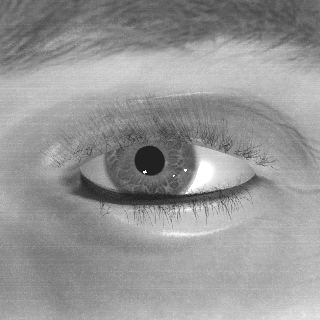
\includegraphics[width=0.3\textwidth]{banana.png}
\end{figure}

\subsection{Convergence of GANs}
Convergence analysis from original paper goes here, together with some comments from other papers regarding divergence measure and stuff.

\subsection{\acrshort{gan} variants}
Just write the variations here in plain text.
\subsubsection{NSGAN} Non-saturating GAN.
\subsubsection{BiGAN}
Can utilize the latent space.
\subsubsection{ACGAN}
Generates nice images. \textcite{odena2016conditional} Distribution is skewed. \textcite{shuac2017acganisbad}.
\subsubsection{WGAN}
\subsubsection{BEGAN}
\subsubsection{DRAGAN}
\subsubsection{Progressive GAN}

\subsection{Difficulties when training GANs}
They do not need to decrease a divergence at each step \textcite{fedus2017many}

\subsection{Evaluating the performance of GANs}
Are all GANs created equal? \textcite{lucic2017gans}

Problem with inception score on AC-GAN \textcite{shuac2017acganisbad}



\section{\acrlong{vaes}}
Another popular family of generative models besides \acrshort{gans} are \acrfull{vaes}. \acrlong{vaes} were first introduced by \textcite{kingma2013auto} as a scalable approach for stochastic variational inference. \acrshort{vaes} are trained using the \acrfull{aevb} algorithm proposed in the same article. 

These models consists of an i.i.d. data set $\dataset$ and a continous latent variable $Z$ in a latent space $\latentspace$. The data set is viewed as a set of outcomes of a random variable $S$ as previously. The prior $p(Z)$ and likelihood $p(S|Z)$ are assumed to come from parametric families of distributions and the posterior $p(Z|S)$ is assumed to be intractable and is modeled by some parametric distribution. The parameters of the prior and likelihood distribution are commonly denoted as the generative model parameters $\theta$. The probabilities in the context of these model are commonly denoted as $p_\theta(X)$, $p_\theta(X|Z)$ and $p_\theta(Z|X)$ to explicitly expose the model parameters. Since the posterior $p_\theta(Z|X)$ is assumed intractable it is estimated with a variational approximation, commonly denoted $q_\phi(Z|X)$. From the deep learning perspective, $q_\phi(Z|X)$ is commonly refered to as the \textit{encoder}, and $p_\theta(X|Z)$ is commonly referred to as the \textit{decoder}.

The \acrshort{aevb} algorithm is applied to learn the generative model parameters and infer the optimal variational parameters. It is a type of approximate variational inference and consists of gradient based optimization of an estimatior of the variational lower bound of the marginal likelihood of the data under the current model. In the original article the authors propose the two estimators based on Monte Carlo estimates of expectations:
\begin{equation}
    \begin{aligned}
        \mathcal{L}^A = \frac{1}{L}\sum_{l=1}^L \log p_\theta (X=x^{(i)},Z=z^{(i, l)}) - \log q_\phi (Z=z^{(i, l)} | X=x^{(i)}) ), \\
        \mathcal{L}^B = - D_{KL}(q_\phi (Z | X=x^{(i)}) || p_\theta(Z=z)) + \frac{1}{L}\sum_{l=1}^L \log p_\theta (X=x^{(i)},Z=z^{(i, l)}).
    \end{aligned}
\end{equation}

\begin{algorithm}
    \caption{Training scheme for \acrlong{vaes}}
  \label{alg:VAEbase}
  \begin{algorithmic}[1]
    \STATE operation 0 \label{op0}
    \STATE operation 1 \label{op1}
  \end{algorithmic}
\end{algorithm}

\begin{figure}
    \caption{Variational autoencoder}
    \label{fig:VAE}
    \centering
    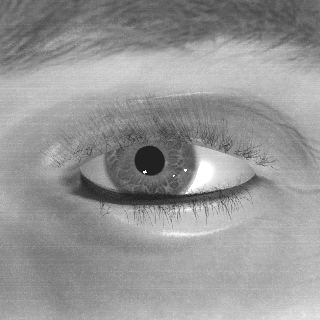
\includegraphics[width=0.3\textwidth]{banana.png}
\end{figure}

\acrshort{vaes} can be trained by maximizing either of these estimates using common gradient based methods as described in Algorithm \ref{alg:VAEbase}. An issue at the moment is that the lower bound estimates require sampling from the latent variable, which is a non-differentiable operation. \textcite{kingma2013auto} resolved this issue by introducing a reparametrization trick to enable gradients to flow through the sampling process. This is applied in Algorithm \ref{alg:VAEbase}, but will not be explained in detail in this report for brevity. The illustrations in \parencite{doersch2016tutorial} are an excellent source of intuition why this works.

\subsection{Similarities with \acrshort{gans}}
Both \acrshort{vaes} and \acrshort{gans} implicitly model the data distribution $p_S(x)$ by introducing a latent stochastic variable Z


\section{Semi-supervised learning}
Formulate problem, go through some apporaches.

Improved GAN, go through vanilla version and combination with self training \cite{wuliu2017selftrainsemisup}

\section{Image-to-Image Models}

\section{Common architectures}

\section{Normalization techniques}

\section{Related work}
Hmm, värt att nämna? 






